\documentclass[a4paper, 11pt]{scrreprt}

\usepackage{fontspec}
\setmainfont{Linux Libertine O}
\usepackage{polyglossia}
\usepackage{amsmath}
\usepackage[hyperref]{xcolor}
\usepackage{graphicx}
\usepackage{listings}
\usepackage{caption}
\usepackage{wrapfig}
\usepackage{float}
\usepackage{booktabs}
\usepackage{numprint}
\usepackage{hyperref}

\newcommand\wiki{\textsc{Wikipedia}}
\newcommand\ew{\textsc{English Wikipedia}}
\newcommand\sew{\textsc{Simple English Wikipedia}}
\newcommand\tableref[1]{\hyperref[#1]{Table \ref*{#1}}}
\newcommand\figureref[1]{\hyperref[#1]{Figure \ref*{#1}}}

\renewcommand\chaptername{Section}
\renewcommand\thechapter{\Roman{chapter}}

\DeclareGraphicsExtensions{.png, .jpeg, .jpg, .svg, .eps}
\graphicspath{{./img/}}

\hypersetup{
  colorlinks = true,
  linkcolor = violet,
  urlcolor = teal,
  citecolor = gray
}

\begin{document}
\begin{titlepage}
  \begin{center}
    \noindent\rule{\textwidth}{0.4pt}
    {\huge\bfseries Improving text readability using\\
      \sew\\}
    \noindent\rule{\textwidth}{0.4pt}\\
    % ----------------------------------------------------------------
    \vspace{1.5cm}
    {\large
      \textbf{Author:} \textsc{Hugo Mougard}
      \hfill
      \textbf{Advisor:} \textsc{Akiko Aizawa}}\\[5pt]
    % ----------------------------------------------------------------
    \vfill
    \parbox{0pt}{\large \begin{tabbing}
        \textbf{Sending institution:} \= National Institute of Informatics \kill
        \textbf{Sending institution:} \> Université de Nantes, France \\
        \textbf{Hosting institution:} \> National Institute of
        Informatics, Japan \\
      \end{tabbing}}
    \vfill
    {\LARGE ATAL Master 2 internship report}
    \vfill
    % ----------------------------------------------------------------
    
\includegraphics[width=0.16\textwidth]{img/nii.png}
    \hfill
    \hfill
    
\includegraphics[width=0.19\textwidth]{img/lina.png}
    \hfill
    
\includegraphics[width=0.19\textwidth]{img/univ.eps}
    \vfill
    {July 2014}
  \end{center}
\end{titlepage}

\tableofcontents

\chapter{Acknowledgments}

I would like to start those acknowledgments with Greg who has to bear
with me for the whole period of this internship. I am grateful for
having a friend around during this internship in Japan, both to enjoy
the trip and discuss many things over the course of those five months.

I also thank Aizawa-sensei and Katsu-san for their precious help
before our arrival to Japan, and their support during our stay.

I wouldn't have been able to conduct this internship without the
scientific advising of Aizawa-sensei and Pascual-san, I thank them for
all their good insight, even though I am convinced I didn't make the
best of it.

Finally I would like to thank Colin de la Higuera for helping from far
away. It was very nice to have someone responsive to discuss the
internship when I wanted to.

\chapter{Laboratory presentation}

\section{National Institute of Informatics}
\label{sec:national-institute-of-informatics}

This internship is taking place at the National Institute of
Informatics in Tokyo, Japan.

\section{Aizawa Laboratory}
\label{sec:aizawa-laboratory}

The team that welcomed me for this work is Aizawa Laboratory. It is
led by Professor Akiko Aizawa. At the time of this writing, the
laboratory has 18 members and strong partnerships with ex-members of
the laboratory.

Its expertise lies in several sub-domains of NLP: gaze-NLP, Analysis
and mining of scientific papers, mathematical information retrieval,
etc.

The work presented in this report has been done in the gaze-NLP
work group. It is so despite the fact that finally no gaze information
was used in the developed approach, because readability has very
strong connections with gaze NLP research.

\chapter{Introduction}

Whether it is to teach children how to read or to assess the
comprehensiveness of technical manuals, readability has been studied
for around two centuries for its impact in both engineering and
scientific endeavors.

Despite this interest of the scientific community, the approaches
proposed have for a long time focused on simple readability
formulas. It is only in recent years that scientists have been able to
come up with more interesting methods, leveraging both the speed of
modern computers and the unparalleled amount of data available on the
internet.

The focus of this internship is to improve on those methods. To be
more specific, most methods consider documents as a whole when
analyzing their readability, which makes it hard for users to
understand which parts are the most important to rework. We aim at
providing a fine-grained analysis of readability in this work. In the
same way than the recursive approach to sentiment analysis
\cite{socher2013recursive} allows users to detect which parts of a
sentence convey which sentiment, we aim at detecting which parts of a
sentence are readable or non readable, and for which reasons.

\chapter{Prior art}
\label{sec:sota}

Readability as been studied extensively. The first works in this area
date back to more than a century ago: in 1893, Sherman published a
book \cite{sherman1893analytics} where he compared modern English and
English spoken four centuries before with considerations that are very
alike the ones that current readability studies outline. Then, in
1921, Thorndike computed a list of ten thousand easy-to-read words
\cite{thorndike1921teacher}. This list got used shortly thereafter by
teachers trying to select good books for children learning to read
\cite{lively1923method}: they went through the process of estimating
the readability of many books thanks to a basic formula and
Thorndike's list.

This was the beginning of an important branch of research focusing on
how to best estimate the readability of a text thanks to simple
formulas. Among the most famous methods, it is interesting to mention
the Flesch Reading Ease \cite{flesch1948new} which introduced the use
of a combination of the average number of words per sentence and the
average number of syllables per word to estimate the readability of a
text, because most of the subsequent approaches also use those
metrics. This method yields a 0.91 correlation with text understanding
and has been used outside of research to improve the readability of a
vast amount of publications, yielding excellent results in readership
increase.

Roughly at the same time, Dale and Chall introduced a readability
formula that uses a list a words instead of the average number of
syllables per word to estimate readability
\cite{dale1948formula}. This more precise definition of world
difficulty allows this metric to reach a 0.93 correlation with text
understanding and because of that has been one of the most used
formulas in research.

Later works brought formulas that are easier to compute or give
slightly better results. Some also give their result as the grade that
would be required to be able to read the input text. Overall are all
using the same variables as either Flesch or Dale and Chall
\cite{mclaughlin1969smog, kincaid1975derivation,
  chall1995readability}.

Despite their useful applications, readability formula are not
perfect. Some works have detailed their problems convincingly, such as
\cite{bailin2001linguistic}

More recently, from 2006 onwards, \sew has been
rightly seen as an important resource for readability studies. Many
scientists have used it to compute parallel corpora of readable their
hard-to-read counterparts sentences.

\chapter{Work}
\label{cha:work}

To address the lack of corpora and tooling in the readability domain,
we propose a method to easily build a parallel corpus using \sew's
revision history. This approach is not novel, since 2008, researchers
have used \sew's revision history to great effect
\cite{nelken2008mining}. What is novel is that we plan on releasing
the corpus with a permissive license and associated tooling to reduce
the entry cost of readability research and allow comparison between
methods on a level ground.

To be able to correctly investigate fine-grained readability, we
propose a software suite to represent results of readability system in
a way that suits analysis.

Finally we experiment with lexical re-writings using our system.

Details on those three main axes follow.

\section{Automatic readability parallel corpus creation}
\label{sec:corpus}

Machine learning approaches have an enormous need for data. Moreover,
they often require a lengthy and costly annotation process. For this
reason, researchers in every domain using machine learning invest time
finding clever techniques to automatically obtain annotated corpora.

In readability, such a clever technique is to leverage the power of
\wiki, and in particular \sew. To do so, mainly two techniques have
been used: the first is to use the articles present both in the
regular \ew{} and in \sew{} and use their comparison as a starting
point to build a parallel corpus. The second is to use the revision
history of \sew. In this work we use the second approach.

When editing \sew, contributors have the possibility to write a commit
message, so that other people can quickly browse history and guess the
role of a particular commit. Using a method close to the
\textsc{Simpl} approach presented in \cite{yatskar2010sake}, we use
those commits to detect readability-oriented modifications. An example
of such modification can be found in \figureref{fig:dan-kelly}.

\begin{figure}[H]
  \centering
  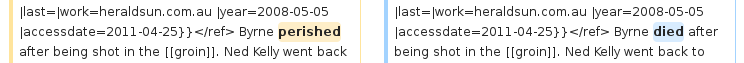
\includegraphics[width=\textwidth]{dan-kelly}
  \caption{An edit of the Dan Kelly article with the commit message
    “use simple english here”}
  \label{fig:dan-kelly}
\end{figure}

However, unlike previous work, we use a very strict heuristic to
reduce the (already important) noise of such a method: we only
consider edits with commit messages $m$ so that:

\[
m \in \left\{\text{“simplify”}, \text{“simplifying”},
  \text{“simplified”}, \text{“simplification”},
  \text{“simpler”}\right\}
\]

This may seem drastic but we believe it is necessary due to the many
noisy commits introduced with broader rules. To illustrate this point,
we can consider the commit messages of
\tableref{tab:problematic-commits}. We can see that commit \#1 has two
purposes, one of which will bring noise (the wikification). Commit \#2
contains one of the matching terms, but we should not consider
it. It's not clear if commit \#3 tries to address readability or not.

Furthermore, we determined by an empirical study that those commits
represented an important part of the commits we might have retrieved
with a broader rule, so we simply did not consider them.

\begin{table}[H]
  \centering
  \caption{Problematic commit messages}
  \begin{tabular}{rp{12cm}}
    \toprule
    \# & Commit message \\
    \midrule
    1 & “simplified, and wikified” \\
    \addlinespace
    2 & “wikify. needs simplifying” \\
    \addlinespace
    3 & “exhaustive, to help us work out titles of articles - lots of
    discussion here, and no, this is not simple engouh yet” \\
  \end{tabular}
  \label{tab:problematic-commits}
\end{table}

The next step for the creation of the corpus is to compute the precise
edit that the contributor made. To do so, we use the uimaFIT
framework\footnote{\url{https://uima.apache.org/uimafit.html}},
OpenNLP preprocessing components
\footnote{\url{https://opennlp.apache.org/}} and jgit's diff
utility\footnote{\url{http://www.eclipse.org/jgit/}} to compute the
difference between the pre- and post- interesting commit versions of
the an article.

The precise pipeline is available on
github\footnote{\url{https://github.com/m09/readability}} and is freely
re-usable.

The obtained unfiltered corpus has \numprint{43753} entries. When
filtered to only consider revisions of 5 words at most, to match the
policy used in \cite{yatskar2010sake}, the number of entries is
reduced to \numprint{23507}.

\section{Fine-grained readability analysis framework}
\label{sec:framework}

Having a parallel corpus available, the next question was to properly
analyze any result derived from it. To properly do that, we went on
and created a web demonstration of an effective visualization of
transformations possible with the corpus.

\section{Automatic rewriting of texts}
\label{sec:rewriting}

\chapter{Open source contributions}
\label{cha:oss-contribs}


\chapter{Conclusions  et perspectives}

\bibliographystyle{apalike2}
\bibliography{report.bib}

\end{document}
%%% Local Variables: 
%%% coding: utf-8
%%% mode: latex
%%% TeX-engine: xetex
%%% End: 
